% Experiments chapter.
%
% Developed for my Master Thesis at Maastricht University.
% Based on Eugenio Senes's template at the University of Torino.
%
% By Joeri Hermans (joeri@joerihermans.com)
%
% Released under an MIT license. Share, modify and enjoy, but quote the author!

\chapter{Experimental Setup}
\label{chapter:experiments}

This chapter describes the experimental setup of our experiments in Chapter~\ref{chapter:accumulated_gradient_normalization} and Chapter~\ref{chapter:asynchronous_distributed_adaptive_gradients}. Furthermore, the architecture of \emph{dist-keras}, which is our Distributed Deep Learning framework based on Apache Spark and Keras, is also introduced.

\section{Distributed Keras}
\label{sec:distributed_keras}

Distributed Keras, or \emph{dist-keras} in short, is a distributed Deep Learning framework built on top of Apache Spark and Keras with the goal to significantly reduce the training using distributed machine learning algorithms, and allow bigger than memory datasets. This project initially started as a prototype with the CMS collaboration. However, the project has seen several iterations since its start in August 2016, and is still undergoing active development~\cite{dist_keras}. Furthermore, \emph{dist-keras} is designed with a focus on "state-of-the-art" distributed optimization algorithms. We designed the framework in such a way that a new distributed optimizer could be implemented with ease, thus enabling a person to focus on research. Several distributed methods are supported, such as, but not restricted to, the training of ensembles and models using data parallel methods.

\subsection{Architecture}
\label{sec:dist_keras_architecture}

Before we dive into the architecture of \emph{dist-keras}, let us first discuss several concepts within Apache Spark, since these are heavily used in the framework. First, Apache Spark is a general purpose cluster computing framework using directed acyclic computation graphs to define a sequence of operations. This graph is constructed by a \emph{driver} program, which responsibilities are to send new instructions to worker nodes, or receive results. However, the driver program does \emph{not execute} any instructions from the DAG (directed acyclic graph). The processes which are responsible for the execution of the DAG, are called \emph{executors}. Usually, executors are spawned dynamically using a cluster resource manager. However, it is possible to spawn them manually on every cluster node with the disadvantage that job-dependent configurations (e.g., memory) are not possible.\\

Nevertheless, an additional important aspect is the way data is handled. Spark usually benefits from a large amount of memory, since it tries to fit as much as possible data in memory to increase the processing throughput. However, if the data does not fit in memory, a flag has to be specified to modify the persistance of the data, meaning, data is allowed to be serialized to disk, and read back into memory when needed. Furthermore, since a computation is defined as a DAG, data can be recomputed in the case of a potential loss due to, for example, data not fitting into memory, or serialized data not fitting on a local disk, or even an unexpected shutdown. Furthermore, to prevent a complete recomputation of data, one can \emph{cache} the data at a specific point. Basically, calling \emph{cache} (checkpointing) on a dataset, tells the executors to keep track of the data in its current form, i.e., not recomputing it. Furthermore, in order to apply modifications, or mapping functions to datasets in a distributed manner, Spark provides an abstraction of data in terms of \emph{Resilient Distributed Dataset}. As discussed before, the term \emph{resilient} implies that the data is able to recover from failures described above. Furthermore, Spark also provides some syntactic sugar in terms of DataFrames and DataSets to easily manipulate data in a tabular format. However, in contrast to regular tabular entries, data rows are not limited to a specific schema, but can be customized if desired. As a result, we can construct any particular dataset of interest in a Spark DataFrame, and preprocess it for Deep Learning, or other analytical purposes. Furthermore, since Apache Spark provides several utilities to distribute the data among the executors, and stream the data were needed, an architecture can be constructed to feed the data to Deep Learning models in production, or during training.\\

In general, a \emph{dist-keras} workflow proceeds as follows. Initially, a Keras model is constructed on the machine were the Spark Driver will be allocated, this could be a personal laptop or desktop computer, however, it is recommended that this machine is in nearby proximity of other cluster nodes and has performant hardware including efficient networking capabilities because the parameter server will be allocated on this machine. Nevertheless, despite the fact allocating a single parameter server creates a significant bottleneck on this particular machine, especially when using large models, it proved to be sufficient for our use-cases. However, in essence it should be possible to allocate parameter servers dynamically on different machines since our current parameter server implementations does not have any Spark dependencies. Next, the data is read from a raw datasource, e.g., \emph{csv}, \emph{Apache Parquet}, or \emph{Apache Avro}, or some other data format that is supported. However, at this point the data is spread over several machines, but not all machines involved in the training procedure. To ensure fast delivery of the data to the executor, we \emph{repartiton} the data equal to the number of workers which will train the model in parallel. However, due to Spark's \emph{lazy-evaluation} mechanism, the repartitioning (shuffling) of the data is not triggered. To trigger this, we call a Spark \emph{action} such as a \emph{count}, to execute the DAG computation.

\begin{figure}[H]
  \centering
  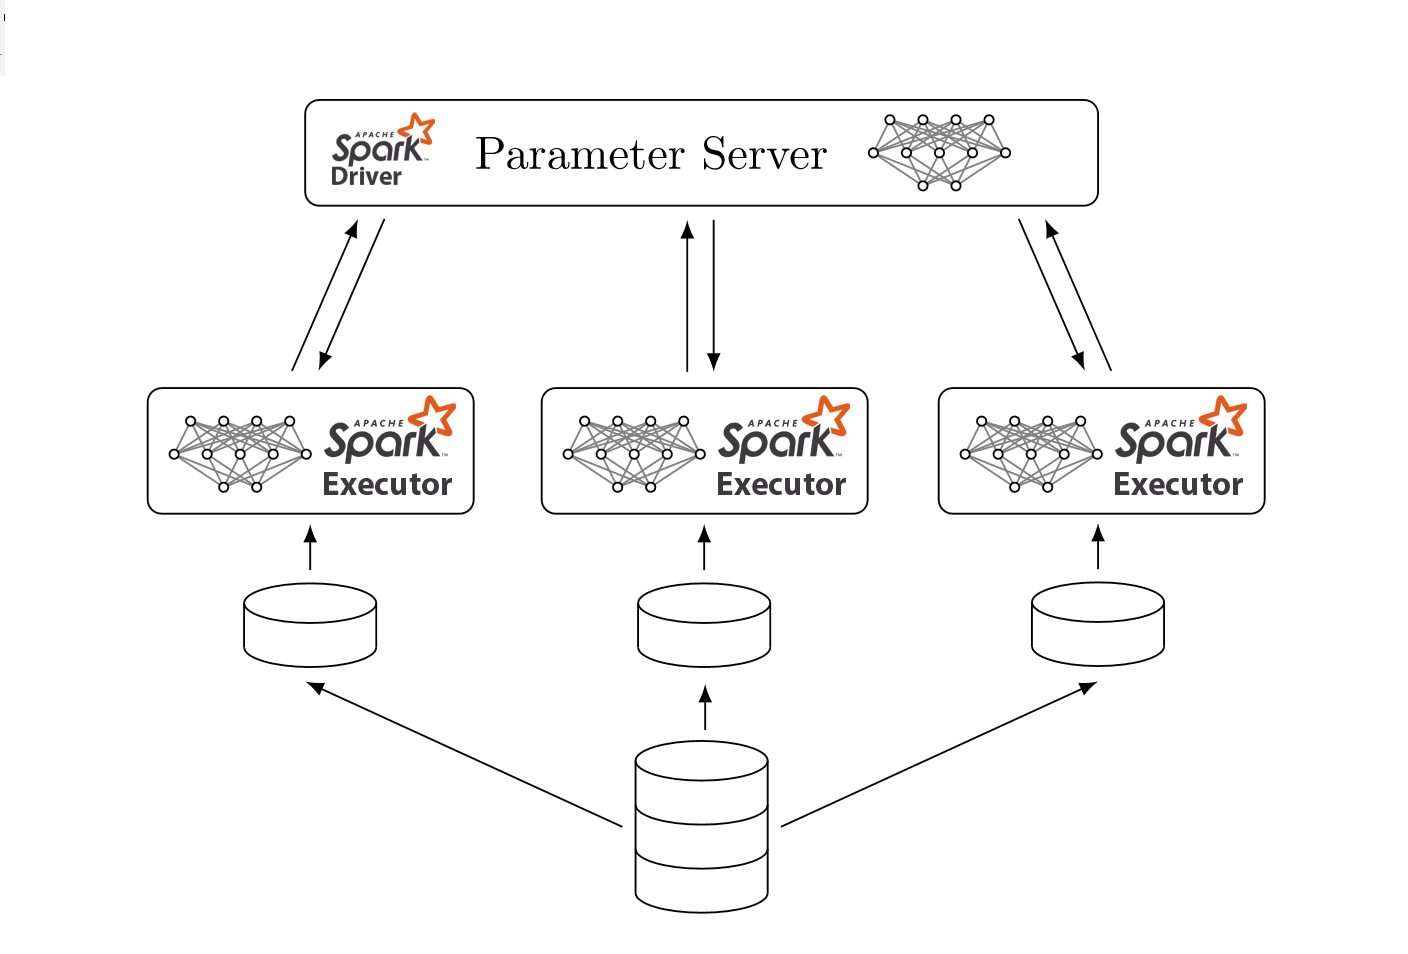
\includegraphics[width=.8\textwidth]{resources/images/dist-keras}
  \caption{Architecture of Distributed Keras and assigned roles during a distributed optimization procedure. As stated before, the Spark Driver will spawn the parameter server on the same machine. However, since our parameter server implementation does not have any Spark dependencies, it can in principle be spawned on any cluster machine.}
  \label{fig:dist_keras_architecture}
\end{figure}

Before starting the training procedure, all relevant objects such as model weights, optimizer, input column, output column, and so on, are serialized. After the serialization of the training configuration is done, the configuration is transported to the Spark executors, where they can be deserialized and reinstantiated. At this point, two concurrent threads will be spawned on every executor. The first thread is responsible for the prefetching of the data, since it is possibly that the data needs to be streamed from a different machine. Furthermore, this thread is also responsible for converting the prefetched training samples into the expected format, i.e., \emph{numpy matrices}. The second thread is mainly responsible for the training procedure, shown in Figure~\ref{fig:dist_keras_architecture}. This thread will implement a specific distributed optimization procedure such as \textsc{adag-agn}, \textsc{aeasgd}, or \textsc{downpour}. Nevertheless, during the training procedure, every worker will collect a set of timestamped training metrics (batch accuracy, batch loss). Meaning, after every computation of a mini-batch, the training metrics are timestamped and yielded to Spark for later processing. After all data has been processed, training metrics of all Spark executors are collected and processed to generate central variable accuracy and loss over time.\\

Finally, when the DAG computation is completed, \emph{dist-keras} fetches the most recent parameterization from the parameter server, and initializes a model with that parameterization. Afterwards, a user can potentially compute validation accuracy in a distributed manner since several utility data \emph{transformers} and \emph{predictors} are provided by \emph{dist-keras}.

\section{Use-case: CMS Event Identification}
\label{sec:experiment_track_reconstruction}

To reduce the computational load of collision reconstructions in future LHC runs, the CMS experiment is exploring Machine Learning techniques as a possible approach for accomplishing this. In this particular case, the experiment is evaluating Deep Learning techniques by fitting them to physics problems. High-level problems such as deciding which data to keep in the High Level Trigger given some physical attributes, and other inference problems, are possible applications. Not because of a statistical perspective perce, but mostly to reduce computational complexity. In the following experiments, we mainly occupy ourselves with the reconstruction of \emph{particle tracks}, and identification of \emph{track types} from raw detector \emph{hits}. A particle track, \emph{track} denoted from this point on, is the path that has been traversed by a particle through the detector. The track is reconstructed from a set of hits, which have been triggered (detected) by parts of the detector. The reconstruction of these tracks is a computationally intensive process, since given a set of hits, one needs to minimize the $\chi^2$ error of the track with respect to the set of hits that have been associated with a particular track. However, this is only one aspect of the problem, one first needs to obtain the set of hits which describe a track given all hits within a collision, which also includes the background (false-positives) generated by the detector itself. Currently, the set of hits related to a single track are extracted using a two-pass Kalman filter and a iterative method to find the best fit, with the first pass of the Kalman filter starting on the outer edges of the detector.\\

An additional problem of applying Deep Learning, or any other Machine Learning approach to the problem of track reconstruction, or event identification, is the petabyte scale data that needs to be dealt with. A simple, and more common solution would be to sample a more manageable fraction of the dataset to train our models on. However, we want the model to be able to extract as many diverse tracks as possible that have been reconstructed over previous years by reconstruction software. As a result, a distributed (data parallel) approach is necessary. However, the data representation is also an important aspect of the problem. Currently, all collisions are stored in the \textsc{root} format, where every reconstructed track for a particular collision (or set of collisions), including the hits of the track, and track parameters can be extracted from. This specific data format is quite problematic, especially taking the petabyte-scale data into account. Furthermore, depending on the modelling, the data needs to be preprocessed in a particular way. One could of course preprocess the complete physics data in a format, shape the data accordingly, and simply copy the data to the machines which will be used during training. However, this is not a very space efficient approach.\\

A more reasonable, and space efficient approach would be to deliver the preprocessed data to the training procedure in a streaming manner. For example, every worker has a buffer in which it will prefetch and preprocess data coming from the \textsc{root} format in a way the model will understand, e.g., \emph{numpy} arrays. This approach does not have the space inefficiencies the previous approach had. However, there is an increased computational load on the worker nodes due to the prefetching, preprocessing of the data, and duplicate processing of the same training samples if multiple epochs of training are required. Nevertheless, compared to computation of gradients in large models, this load is neglectable. An additional benefit of this approach is that the same architecture can be used during model development, since data representations can be generated on-the-fly as in Apache Spark, shown in Figure~\ref{fig:experiment_cms_tracking}.

\begin{figure}[H]
  \centering
  \begin{subfigure}{.48\textwidth}
    \centering
    \includegraphics[width=\linewidth]{resources/images/experiment_cms_tracking_1}
    \caption{Low $p_T$ (transverse momentum)}
    \label{fig:experiment_cms_input_1}
  \end{subfigure}
  \begin{subfigure}{.48\textwidth}
    \centering
    \includegraphics[width=\linewidth]{resources/images/experiment_cms_tracking_2}
    \caption{High $p_T$, very dense point cloud.}
    \label{fig:experiment_cms_input_2}
  \end{subfigure}
  \caption{Pixel-binned data representation of the hits which occurred in two different collisions.}
  \label{fig:experiment_cms_tracking}
\end{figure}

Therefore, in a final system architecture, we could combine several ideas presented in this thesis to build is system which is able to handle such a data-scale.
